\documentclass[10pt,a4paper]{article}
\usepackage[utf8x]{inputenc}
\usepackage[T1]{fontenc}
%\usepackage{stringenc} % for grffile
\usepackage{ucs}
\usepackage{amsthm} %numéroter les questions
\usepackage[english]{babel}
\usepackage{datetime}
\usepackage{xspace} % typographie IN
\usepackage{hyperref}% hyperliens
\usepackage[all]{hypcap} %lien pointe en haut des figures
\usepackage[english]{varioref} %voir x p y
\usepackage{fancyhdr}% en têtes
%\input cyracc.def
\usepackage[]{graphicx} %include pictures
%\usepackage[encoding,inputencoding=utf8,filenameencoding=utf8]{grffile}
%\usepackage[extendedchars,inputencoding=latin1,filenameencoding=latin1]{grffile}
\usepackage[siunitx ]{circuitikz}
%\usepackage{gnuplottex}
\usepackage{ifthen}
\graphicspath{{./figures/}}
\usepackage{array}
\usepackage{amsmath}
\usepackage[]{xcolor}
\usepackage{tikz}
\usepackage{tikz-timing}
\usetikzlibrary{scopes}
\usetikzlibrary{backgrounds}
\usepackage{listings}
\usepackage{enumitem}
\usepackage[top=1 in, bottom=1 in, left=1.3 in, right=1 in]{geometry} % Yeah, that's bad to play with margins
\usepackage[]{pdfpages}
\usepackage{pdflscape}
\usepackage[]{attachfile}
\usepackage{colortbl}
\usepackage{multirow}
\usepackage{booktabs}
\usepackage{rotating}
\usepackage{fontawesome} %Symbols

\newcommand{\version}{v1.0.2}

%cyr
%\newcommand\textcyr[1]{{\fontencoding{OT2}\fontfamily{wncyr}\selectfont #1}}


\newboolean{corrige}
%\setboolean{corrige}{true}%corrigé
\setboolean{corrige}{false}% pas de corrigé

\usepackage{aeguill} %guillemets

%% fancy header & foot
\pagestyle{fancy}
\lhead{[ELEC-H-473] Microprocessor Architectures: TIS-100}
\rhead{\version\\ page \thepage}
\chead{\ifthenelse{\boolean{corrige}}{Corrigé}{}}
\cfoot{}
%%

\pdfinfo{
/Author (La saucisse électronique volante)
/Title (ELECH473 Lab 6 - TIS-100)
/ModDate (D:\pdfdate)
}

\hypersetup{
pdftitle={ELECH473 Lab 6 - TIS-100},
pdfauthor={Mouette unijambiste vengeresse},
pdfsubject={TIS-100}
}

\theoremstyle{definition}% questions pas en italique
\newtheorem{Q}{Question}[] % numéroter les questions [section] ou non []

\newcommand{\reponse}[1]{% pour intégrer une réponse : \reponse{texte} : sera inclus si \boolean{corrige}
	\ifthenelse {\boolean{corrige}} {\paragraph{Réponse :} #1} {}
 }

\newcommand{\addcontentslinenono}[4]{\addtocontents{#1}{\protect\contentsline{#2}{#3}{#4}{}}}

\newcommand{\on}[1]{{\operatorname{#1}}}

\def\labelitemi{--}
\setlist{parsep=0pt,itemsep=0pt,style=standard,leftmargin=\parindent, align=left} % pas d'espace prohibitif entre les items
\setlist{nolistsep}

\newcolumntype{C}[1]{>{\centering\let\newline\\\arraybackslash\hspace{0pt}}m{#1}}

\setlength{\tabcolsep}{0pt} %no extra space in cells to keep constant tabular width

\date{\vspace{-1cm}\version}
\title{\vspace{-2cm} Lab 6\\ Microprocessor Architectures [ELEC-H-473]\\ Tessellated Intelligence System \ifthenelse{\boolean{corrige}}{~\\Corrigé}{}}

%\author{\vspace{-1cm}}%\textsc{Yannick Allard}}


\lstdefinestyle{customasm}{
 % belowcaptionskip=1\baselineskip,
 % frame=L,
 % xleftmargin=\parindent,
  language=[x86masm]Assembler,
  basicstyle=\footnotesize\ttfamily,
  commentstyle=\itshape\color{magenta!40!black},
   comment=[l]//,
}

\lstset{escapechar=@,style=customasm}

\begin{document}

% Introduce a new counter for counting the nodes needed for circling
\newcounter{nodecount}
% Command for making a new node and naming it according to the nodecount counter
\newcommand\tabnode[1]{\addtocounter{nodecount}{1} \tikz \node (\arabic{nodecount}) {#1};}

% Some options common to all the nodes and paths
\tikzstyle{every picture}+=[remember picture,baseline]
\tikzstyle{every node}+=[inner sep=0pt,anchor=base]
\tikzstyle{every path}+=[thick, rounded corners]



\maketitle
\section*{Introduction}

Using an exclusive architecture, we want to show you:
\begin{itemize}
\item how to train to quickly digest a new architecture documentation and get productive quickly;
\item how to optimize your code under heavy hardware constraints;
\item that it is possible to learn and play at the same time.
\end{itemize}
~\\

What you will need:
\begin{itemize}
\item A copy of TIS-100 (DRM-free from the lab network drive (Z:/))
\item The TIS-100 reference manual
\item RTFM
\end{itemize}
~\\
If you like this lab and want to continue playing, consider supporting the developers by buying the game on Steam (DRM-free key available at \href{https://www.humblebundle.com/store/tis100}{Humble Bundle})

\section{Tessellated Intelligence System: TIS-100}
You are a system engineer charged with completing a set of tasks on an old computer: the TIS-100.
Its architecture is composed of twelve interconnected nodes that can exchange data with their direct neighbours.
Each node can be one out of the three possible types: 
\begin{itemize}
	\item Regular computing node
	\item Memory stack node
	\item Corrupted and unusable node
\end{itemize}

\subsection{Computing node}
\begin{center}
	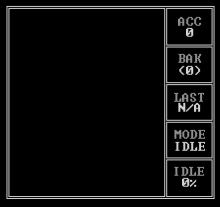
\includegraphics[width=4cm]{computing-node.png}
\end{center}

The node is composed of a 15-lines programmable area surrounded by its register and various information.
It has two registers: \texttt{ACC} and \texttt{BAK}, the former being directly addressable whereas the later and can only be modified using the \texttt{SAV} and \texttt{SWP} commands.
The \texttt{LAST} register tells you which port has been used last, \texttt{MODE} what the node is doing and \texttt{IDLE} the percentage of time the node has spent doing nothing.

Using the \texttt{MOV} instruction, it can communicate with the surrounding computing or memory stack nodes.



\subsection{Memory stack}
\begin{center}
	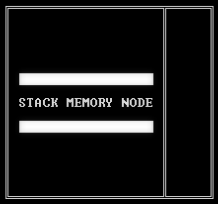
\includegraphics[width=4cm]{memory-stack-node.png}
\end{center}

The memory stack node, as its name indicates is a stack in which the first element added is the last that can be accessed.
Such a structure is also called ``last in, first out", or LIFO.

The content of the node can be accessed using the \texttt{MOV} instruction.




\subsection{Instruction set}
The instruction set only contains a handful instructions such as addition, substraction and a bunch of comparison against zero.
The full set is detailed in the reference manual, but the general idea is
\begin{center}
	\verb!<instruction> <source>, <destination>!
\end{center}

Please note that although the reference manual says so, there is no ``model-specific manual" nor ``Tessellated Intelligence System Best Practices *" extra documents.

\subsection{Use custom specifications}
The game comes with a bunch of levels you need to solve in order to complete the game.
However, you can also create your own levels using the specification editor.

You can import custom levels by copying the corresponding \texttt{.lua} files into the right folder depending on your operating system:
\begin{itemize}
	\item[\faWindows] \verb|My Documents\My Games\TIS-100\<UID>\custom|
	\item[\faLinux] \verb|$HOME/.local/share/TIS-100/<UID>/custom|
\end{itemize}
where \texttt{<UID>} is either \texttt{0} if you are using the DRM-free version of the game or your Steam ID if you are playing on Steam.

For this lab, you will need to import three levels:
\begin{itemize}
	\item ``Decode the image" (\texttt{14173819.lua})
	\item ``Coprime detector" (\texttt{69396829.lua})
	\item ``Multiplication" (\texttt{73121466.lua})
\end{itemize}


\section{Your mission}

\subsection{Basics}

We strongly advise you to first train on the pre-existing levels of the game before tackling the custom specifications (see Assignment).
You should get the hang of it by the end of the fourth level: ``Signal comparator".

\subsection{Assignment}
We ask you to solve two custom levels: ``Decode the image" and ``Coprime detector".
The grade will be based on the performance of all the submissions and weighted across the three measures: node, instruction and cycle count.
If you performed better than all the other groups for at least one of the three performance measures, you will get a perfect grade for the exercise, that is two out of two.
Otherwise, you will be awarded one point if the problem is solved and the second point will be weighted against all submissions (e.g. if you performed the worst in all three measures, you won't get any point, if you are right at the average, you will get half a point).

We will not disclose the performance of the submissions before the last group has sent us his submission, as you are not all synchronized.
~\\

\textbf{You will need to send us two \text{.txt} files, one for each solution.}

Those save files can be found in:
\begin{itemize}
	\item[\faWindows] \verb|My Documents\My Games\TIS-100\<UID>\save\<solution_file>|
	\item[\faLinux] \verb|$HOME/.local/share/TIS-100/<UID>/save/<solution_file>|
\end{itemize}
where \texttt{<solution\_file>} follows this syntax: \texttt{SPEC<specification ID>.<solution number>.txt}.

For example, a solution to the ``Decode the image" problem can be found under the name \texttt{SPEC14173819.0.txt}.

Do \textit{not} change the file name when sending it to us.
If you are not sure you are selecting the right file, just open it and check its content.

% \begin{Q}
% \end{Q}

\end{document}
